%%%%%%%%%%%%%%%%%%%%%%% file template.tex %%%%%%%%%%%%%%%%%%%%%%%%%
%
% This is a general template file for the LaTeX package SVJour3
% for Springer journals.          Springer Heidelberg 2010/09/16
%
% Copy it to a new file with a new name and use it as the basis
% for your article. Delete % signs as needed.
%
% This template includes a few options for different layouts and
% content for various journals. Please consult a previous issue of
% your journal as needed.
%
%%%%%%%%%%%%%%%%%%%%%%%%%%%%%%%%%%%%%%%%%%%%%%%%%%%%%%%%%%%%%%%%%%%
%
% First comes an example EPS file -- just ignore it and
% proceed on the \documentclass line
% your LaTeX will extract the file if required
\begin{filecontents*}{example.eps}
%!PS-Adobe-3.0 EPSF-3.0
%%BoundingBox: 19 19 221 221
%%CreationDate: Mon Sep 29 1997
%%Creator: programmed by hand (JK)
%%EndComments
gsave
newpath
  20 20 moveto
  20 220 lineto
  220 220 lineto
  220 20 lineto
closepath
2 setlinewidth
gsave
  .4 setgray fill
grestore
stroke
grestore
\end{filecontents*}
%
\RequirePackage{fix-cm}
%
%\documentclass{svjour3}                     % onecolumn (standard format)
%\documentclass[smallcondensed]{svjour3}     % onecolumn (ditto)
\documentclass[smallextended]{svjour3}       % onecolumn (second format)
%\documentclass[twocolumn]{svjour3}          % twocolumn
%
\smartqed  % flush right qed marks, e.g. at end of proof
%
\usepackage[utf8]{inputenc}
\usepackage{longtable}
\usepackage{graphicx}
\usepackage{hyperref}
\usepackage[usenames,dvipsnames]{color}
\usepackage{natbib}
\usepackage{lscape}
\usepackage{float}

%
% \usepackage{mathptmx}      % use Times fonts if available on your TeX system
%
% insert here the call for the packages your document requires
%\usepackage{latexsym}
% etc.
%
% please place your own definitions here and don't use \def but
\newcommand{\jri}[1]{{\small \textcolor{blue}{\bf #1}}}
\newcommand{\pb}[1]{{\small \textcolor{Tan}{\bf #1}}}

%
% Insert the name of "your journal" with
% \journalname{myjournal}
%
\begin{document}

\title{Diversity and evolution of centromere repeats in the maize genome%\thanks{Grants or other notes
%about the article that should go on the front page should be
%placed here. General acknowledgments should be placed at the end of the article.}
}
%\subtitle{Do you have a subtitle?\\ If so, write it here}

%\titlerunning{Short form of title}        % if too long for running head

\author{Paul Bilinski \and Kevin Distor \and Jose Gutierez-Lopez \and Gabriela Mendoza Mendoza \and Jinghua Shi \and Kelly Dawe \and Jeffrey Ross-Ibarra}

%\authorrunning{Short form of author list} % if too long for running head

\institute{Paul Bilinski : Kevin Distor : Jose Gutierez-Lopez : Gabriela Mendoza Mendoza : Jeffrey Ross-Ibarra\at
              Department of Plant Sciences, UC Davis\\
              Davis, California, 95616
              \and
              Jeffrey Ross-Ibarra\at
              The Genome Center and Center for Population Biology, University of California\\
              Davis, California, 95616\\
              \email{rossibarra@ucdavis.edu}           %  \\
%             \emph{Present address:} of F. Author  %  if needed
           \and
           Jinghua Shi : R. Kelly Dawe\at
           Department of Plant Biology, University of Georgia\\
	  Athens, Georgia, 30602
           \and
           R. Kelly Dawe\at
           Department of Genetics, University of Georgia\\
           Athens, Georgia, 30602\\
}

\date{Received: date / Accepted: date}
% The correct dates will be entered by the editor
\maketitle

\begin{abstract}

Centromere repeats are found in most eukaryotes and play a critical role in kinetochore formation.  Though they exhibit considerable diversity both within and among species, little is understood about the mechanisms that drive centromere repeat evolution.  Here, we use maize as a model to investigate how a complex history involving polyploidy, fractionation, and recent domestication has impacted the diversity of the maize CentC repeat.  We first validate the existence of long tandem arrays of repeats in maize and other taxa in the genus \emph{Zea}.  We find that genetic similarity among CentC copies is highest within these arrays, suggesting that tandem duplications are the primary mechanism for the generation of new copies.  In spite of this, we see little evidence that CentC variants form distinct genetic groups, instead finding that homoplasious mutations have likely homogenized CentC diversity.   Although the two ancestral subgenomes of maize have contributed nearly equal numbers of centromeres, our analysis shows that a vast majority of all CentC repeats derive from only one of the parental genomes.  Finally, by comparing maize with its wild progenitor teosinte, we find that the abundance of CentC, but not the pericentromeric repeat Cent4, has decreased through domestication. 

\keywords{Centromere \and Evolution \and Subgenome}
% \PACS{PACS code1 \and PACS code2 \and more}
% \subclass{MSC code1 \and MSC code2 \and more}
\end{abstract}

\section*{Introduction}
\label{intro}
In spite of the rapid growth of sequenced plant genomes, plant centromeres remain poorly understood and relatively cryptic, due largely to their highly repetitive content.  Centromere repeats are highly diverse across taxa and their turnover appears to be very rapid \citep{Melters2012}. However, little is known about the genetic mechanisms that produce centromere repeat diversity.  
Domesticated maize (\emph{Zea mays} ssp. \emph{mays}) has a high quality genome assembly \citep{Schnable2009} including complete sequence of two centromeres \citep{Wolfgruber2009}, and the breadth of research into maize centromeres makes it one of the best systems in which to investigate the processes governing centromere repeat evolution.

Maize centromeres are comprised primarily of the 156bp satellite repeat CentC and the CRM family of retrotransposons.  Both repeats interact with  kinetochore proteins such as CENH3 \citep{Wolfgruber2009, Zhong2002} and show  variation in  abundance across taxa \citep{Albert2010}.  But while there is considerable effort in investigating the molecular function of maize centromere repeats \citep{Ananiev1998B, Nagaki2003, Wolfgruber2009}, we know comparatively little about the evolution of the sequences themselves. CRM elements are better understood, including the age and insertion preferences of different CRM families \citep{Wolfgruber2009, Sharma2008}.  In contrast, there is no in-depth characterization of the genetic diversity of centromere repeats in the maize genome.  
%  studies \citep{Wang2012} have only examined the flanking sequences to CentC islands despite their known association with functional centromeres.  To date,

In this paper, we describe the patterns of diversity of centromere repeats across the maize genome.  We investigate the genetic diversity of these repeats, including whether the differential ancestry of maize centromeres \citep{Wang2012} has led to chromosome-specific variation similar to that seen in other species \citep{Kawabe2005, Pontes2004} and how genetic relatedness among individual repeats varies spatially across the genome.  We then compare centromere abundance across a number of samples of maize and its wild relative teosinte.  We find that CentC copies do not form genetic groups consistent with ancient whole genome duplications or chromosome specificity, but instead that most of the large blocks of CentC appear to have been inherited from only one of the ancestral subgenomes of maize.  We show higher genetic similarity of CentC repeats within clusters, indicating the predominance of tandem duplications in the formation of new CentC copies.  Lastly, we use low coverage sequencing and cytological analyses data to show that domesticated maize has less CentC than its wild relatives.

\section*{Methods} 
\label{methods}

\subsection*{CentC Repeat Identification and Diversity}

We downloaded 218 previously annotated CentC sequences \citep{Ananiev1998B, Nagaki2003} from Genbank.  We then searched the maize genome (5b60, \url{www.maizesequence.org}) with megaBLAST \citep{McGinnis2004} using the 218 annotated CentCs as a reference.  We kept hits with a length of over 140bp and a minimum bit score of 100.  After meeting the bit score threshold, the longest hit was retained.  We defined CentC’s as being in tandem if the CentC’s start location was within 1000bp of the start location of another CentC.
	
All 12,162 CentC sequences were aligned using 7 iterations of Muscle \citep{Edgar2004} with default parameters.  A Jukes-Cantor distance matrix of all sequences was calculated with PHYLIP (\citep{Felsenstein1989} \url{http://evolution.genetics.washington.edu/phylip.html}), and an unrooted neighbor joining tree was built based on the distance matrix.  
	
We used principle coordinate analysis (PCoA) to cluster CENTC variants based on their genetic distances. Eigenvalues from the PCoA were used to determine the number of statistically significant clusters using the Tracy-Widom distribution \citep{Patterson2006}.  
	
We employed the software SpaGeDi (\citep{Hardy2002}\url{http://ebe.ulb.ac.be/ebe/Software.html}) to estimate the spatial autocorrelation of sequence similarity of CENTC repeats in the completely sequenced centromeres 2 and 5.  We calculated Moran’s I statistic using Jukes-Cantor genetic distance and measures of physical distance between CENTC repeats in base pairs.  Confidence intervals for the values of I were estimated by 20,000 random permutations of the physical distances.  
	
Statistical analyses were performed in R with the packages ape \citep{Paradis2004} and RMTstat \citep{Perry2009}.  We compared clusters to chromosome of origin and syntenic maps of maize ancient tetraploidy \citep{Schnable2011} to determine if the genetic history of maize left a footprint on CentC similarity.

\subsection*{Read Mapping and Genome Size Correction}
	
We mapped Illumina reads from a broad panel of \emph{Zea} species \citep{Chia2012,Tenaillon2011}  to a reference consisting of the full complement of 12,162 CentC variants identified in the B73 genome.  We also used previously published whole genome chromatin immunoprecipitation (ChIP) \citep{Wolfgruber2009, Wang2013} with CenH3.  Reads were mapped using  Mosaik v1.0 (\url{https://code.google.com/p/mosaik-aligner/}). We first optimized mapping parameters by relaxing mapping stringency and evaluating the number of successfully mapped reads with each combination.  Consistent with parameters from previous studies mapping reads to repetitive elements \citep{Tenaillon2011}, we required homology to remain at a minimum of 80\%.  For other non-default parameters, we permuted over many values of hash size, alignment candidate threshold,  percent of read aligning, and maximum number of hash positions per seed to find a combination that produced believable alignments.  We selected an optimum combination of parameters just below the parameters where we observed a large increase in the total number of reads aligning (Supplementary Figure \ref{Supp_MPS}).    Our final set of parameters for tandem repeats used an initial hash size of 8, an alignment candidate threshold of 15 bases, 20\% percent of mismatching bases, a minimum of 30\% overlap to the reference, and stored the top 100 hits for alignment.  After reads were mapped, we calculated the percentage of total reads hitting the given reference and multiplied this value by the relative genome size of each accession as reported in \citet{Chia2012} and \citet{Tenaillon2011}. The total number of reads mapping did not change drastically when using one random copy of CentC versus the full AGPv2 reference, suggesting that our parameters are sufficiently broad to capture genome-wide CentC abundances.  Because library preparation has an effect on estimates of repeat abundance (see results), we only used individuals from maize HapMap v2 \citep{Chia2012} with libraries prepared using identical methods.
	
We used a different set of mapping parameters for long repeats such as transposable elements.  Previous studies \citep{Schnable2009} estimated that approximately 85\% of maize genome derives from transposable elements.  Using the short read libraries from \citet{Tenaillon2011}, we selected parameters so that approximately 85\% of the library mapped to the maize transposable element database (\url{www.maizetedb.org}) with a minimum homology of 80\%.  The final parameters for TEs were a hash size of 10, alignment candidate threshold of 11, 80\% homology excluding non-aligned portions of the read, and a 30\% minimum overlap.

We designed a simulation to estimate the accuracy of our measurements of CentC content (code available at: \url{https://github.com/kddistor/dnasims}).  In short, our simulations altered the copy number of CentC repeats over a region of fixed length (10Mb), changing the percentage of the genome deriving from the repeat.  Illumina reads were simulated from each of the DNA strings and mapped using our pipeline.  These simulations showed that our pipeline captured relative differences in abundance well, but underestimated total abundance of CentC.  We found that our pipeline could accurately capture differences of 0.05\% change in CentC abundance, suggesting that larger differences are likely to be biologically real (Supplementary Figure \ref{Supp_Accuracy}).  

\subsection*{Simulation of homoplasious mutations}

%We wanted to better understand the diversity present in all CentC copies across the genome.  Looking at our alignment, we found that the sequences had a pairwise percent identify of 65.8\% with only 2.2\% of sites identical, suggesting large sequence diversity.  However, these statistics do not inform us whether the amount of diversity observed would be expected due to cumulative mutation over time.  
In order to better understand patterns of diversity at CentC, we performed simulations to test the likelihood of homoplasious mutations (i.e. independent mutations occurring at the same position in two different CentC repeats). Our simulation (code available at: \jri{need this github URL!}) assumed that CentC has been evolving for  1 million years since the divergence of maize and \emph{Tripsacum} \citep{Ross-Ibarra2009}, a closely related genus whose centromere repeat shares a large amount of homology \citep{Melters2012}.  We assumed a constant copy number, a mutation rate of $3 x 10^{-8}$ (\jri{CITE Clark 2005 MBE}), and one generation per year.  

\subsection*{PacBio Sequencing}
	
Library preparation and sequencing was performed according to the methods cited in \citep{Melters2012}.  Using those protocols, we sequenced one individual from \emph{mays}, \emph{mexicana}, \emph{parviglumis}, and \emph{Z. luxurians} with Pacific Biosciences (Pacific Biosciences, Menlo Park, CA) technology. Approximately 200Mbp of reads were produced from each cell, and reads with length greater than 600bp were retained for analysis of tandem CentC content using BLAST (Supplementary Table \ref{supp.pacbio}).  CentC copies were considered tandem if the read had 4 CentC copies within 300bp of each other. 

\subsection*{FISH}

Fluorescent in situ hybridization (FISH) was used to compare abundance of CentC repeats in chromosomes of a maize x \emph{parviglumis} F1 hybrid and a maize x \emph{Z. luxurians} F1 hybrid. \jri{Kellyto fill in}	

\section*{Results}
\label{results}
%i imagine results go 1) repeats in the genome. 2) subgenome stuff 3) realtedness (PcoA and spagedi and mutations 4) abundance.

\subsection*{Centromere repeats in the maize genome}

We found a total of 12,162 CentC variants in the maize reference genome and  unassembled BACs.  Of these, 8,259 were unique over their full length. No CentC sequence occurred more than 10 times in the genome, and the vast majority ($>$75\%, Supplemental Table \ref{supp.occurence}) of non-unique CentC variants occurred only twice.  Of the 2,266 non-unique CentC sequences, only 3 were tandem, identical duplicates.  Genome-wide CentC locations also show that nearly all of the 10,639 \jri{why is this different from 8259 number?} CentC copies are found in one of the 248 clusters identified on chromosomes 1-10; only 14 occurred as solo copies.  Clusters varied in width from single CentC copies to 84KB \jri{check is it KB or Kb?}, with a mean of $\sim$7KB ($\sim$45 CentC copies). Chromosomes varied greatly in CentC copy number, though we know that centromere assemblies for all of the chromosomes are not complete.   For example, CENH3-ChIP sequence from an oat-maize addition line including only one maize chromosome \jri{CITE} nonetheless has many reads that map to the unassembled BACs (Supplemental table \ref{gaby}).  In particular, chromosome 6 had many more reads aligning to the unassembled BACs than it did to its own centromere, suggesting a particularly incomplete assembly.  Examining total repeat number, Chromosome 7 had the most CentC, with 3,200 copies, while chromosome 6 had the fewest with 32 copies.  \jri{consistency check: is Chromosome capitalize?}

We used long-read Pacific Biosciences sequencing to verify that most CentC is in tandem arrays. We sequenced whole genome ($\sim 0.1$X) libraries from 4 \emph{Zea} species.  In spite of the low coverage, we recovered reads containing CentC sequence from all four taxa (Supplementary Table \ref{supp.pacbio}).  In one 6.7KB read from the maize reference line B73, for example, we identified approximately 40 independent CentC copies in tandem, and similar arrays were seen in all four \emph{Zea} species analyzed.  These results show that overall structure of the repeats has been maintained for the approximately 140,000 years since the \emph{luxurians}-\emph{mays} divergence \citep{Hanson1996,  Ross-Ibarra2009} and that a majority of CentC is found in tandem arrays (Supplementary Table \ref{supp.pacbio}).

We then identified how many large clusters of CentC were retained from each of the two parental genomes that comprise the extant maize genome, referred to here as subgenome 1 and subgenome 2 (Figure \ref{circos}).  Previous work identified the parental genome for individual chromosomal segments \citep{Schnable2011} and centromeres \citep{Wang2012}.  Because large clusters are less likely to be misassembled, we focused our analyses on the 52 clusters $>$10KB in length (Supplementary Fig \ref{Supp_clusterhist}).  We assign clusters to a subgenome if they are flanked by two regions identified as originating from the same  subgenome.  Thirty-eight of these clusters could be assigned to subgenome 1 (out of 43 assignable). If we restrict the analysis to clusters  $>$20KB, 16 of 17 clusters were unambiguously assigned to subgenome 1.  Even correcting for the genome-wide overrepresentation of subgenome 1 (62.5\% of assigned base pairs), these results suggest a strong inequality in the origin of large CentC clusters (Fisher's exact test, $p<0.005$ for both 10KB and 20KB clusters). \jri{I thought that the 1 large cluster is on chr3 that gernot said is wrong -- if so, can't we claim 17/17 or at least 16/16 assignable?}

\begin{figure}
% For two-column wide figures use
% Use the relevant command to insert your figure file.
%  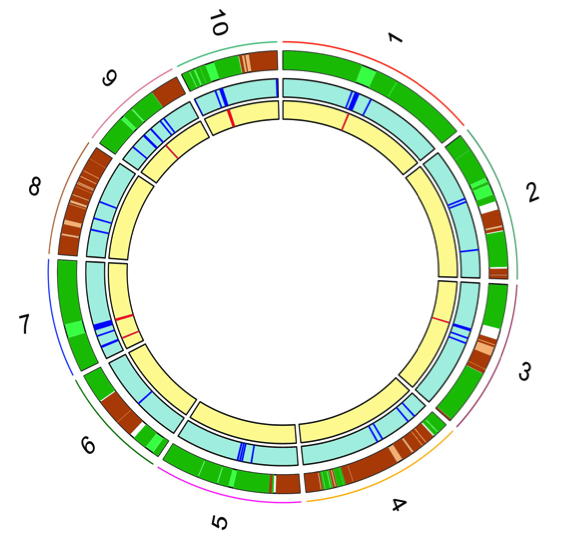
\includegraphics[width=0.75\textwidth]{circos.png}
  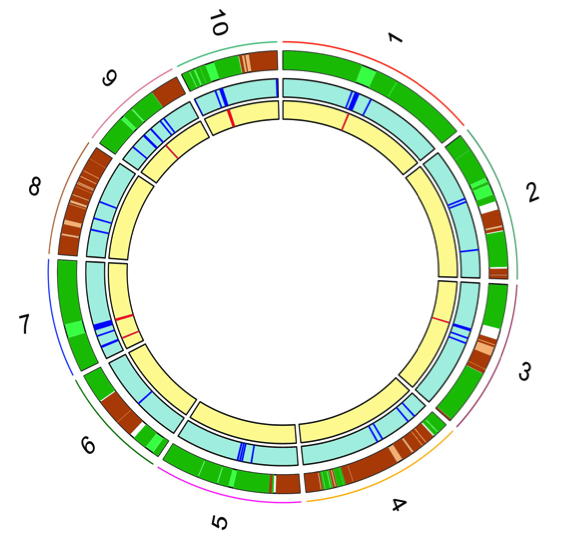
\includegraphics{circos.png}
\caption{CentC repeat location in relation to the maize subgenomes.  The outer ring depicts chromosomal assignment to the two subgenomes, with higher confidence regions are colored with darker colors.  Breakpoints between the subgenomes remain uncolored to indicate uncertainty. The middle ring, shaded in blue, displays the locations of all CentCs across the genome.  The inner ring, shaded in yellow, displays the locations of all CentC clusters greater than 20KB in length.}
\label{circos}    
\end{figure}

In addition to CentC, previous studies have described Cent4, a second high copy number centromere repeat specific to maize chromosome 4 \citep{Page2001}.   BLAST analyses of Cent4 sequences, however, revealed that all 15 had high homology to the poorly characterized LTR retrotransposon RLX\_sela, which was previously shown to be associated with heterochromatic  knobs \citep{Tenaillon2011, Chia2012}.  Whole-genome cenH3 chromatin immuno-precipitation data from  \citet{Wolfgruber2009} shows no significant over-representation of Cent4 compared to five known non-centromeric TE’s. Together, these data suggesting that Cent4 is actually a pericentromeric retrotransposon that is not involved in kinetochore formation on chromosome 4.
	
\subsection*{Relatedness of CentC in the maize genome}

CentC copies in the maize genome exhibit tremendous diversity: the overall pairwise identity in our alignment was only 65\%, and $\sim$98\% of sites in the alignment had at least 2 variants.  Such diversity led us to ask whether genetic groups of CentC variants could be distinguished. We performed principle coordinate  \jri{principal coordinate or principal component?} analyses (PCoA) from a genetic distance matrix estimated from our alignment, and assigned individual repeats to  genetic clusters following the approach of \citet{Patterson2006}.  We found 58 significant clusters, but observed no pattern of groupings that revealed chromosome specificity of CentC’s or the impact of historical tetraploidy (Figure \ref{pcoa}; Supplemental Table \ref{long}).

\begin{figure}[h]
\centering
% For two-column wide figures use
% Use the relevant command to insert your figure file.
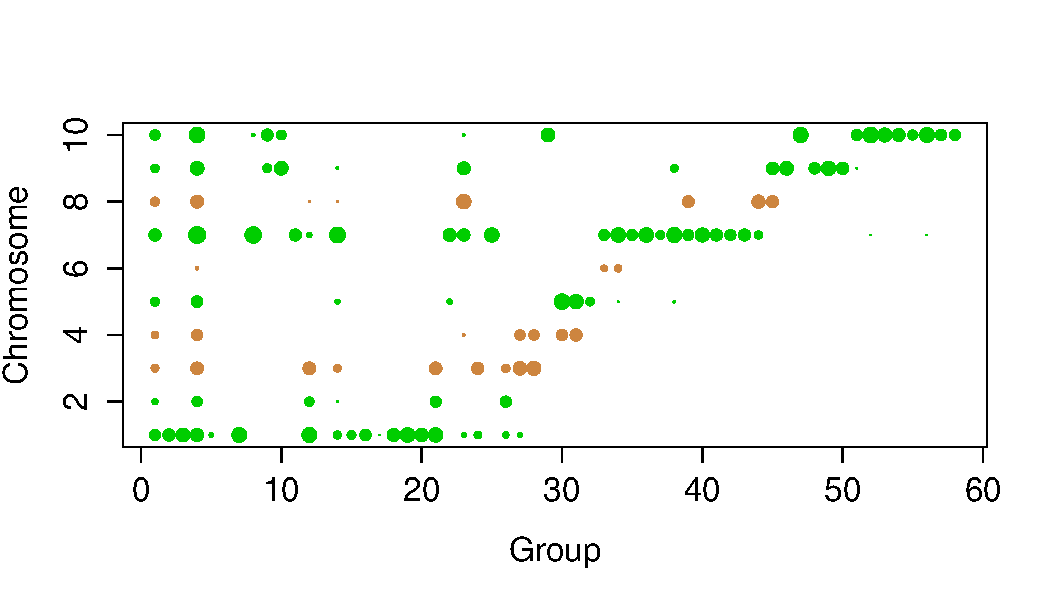
\includegraphics[width=1\textwidth]{Rplot02}
\caption{Presence of CentC in each of the heirarchical groups.  The 58 clusters found to be statistically significant in forming genetic groups are represented on the x-axis and chromosome of origin on the y-axis. The size of each point is proportional to the log number of sequences in that group on that chromosome. CentC counts from chromosomes whose centromeres were derived from subgenome 1 are colored green and those from subgenome 2 are colored brown. 
}
\label{pcoa}    
\end{figure}

The tandem nature of CentC suggests it increases in copy number through local duplications that produce initially identical copies.  This predicts that local clusters of CentC should be more closely related than CentC from different clusters.  Comparisons of genetic and physical distance among CentC repeats on chromosomes 2 and 5 indeed shows this pattern (Figure \ref{heatmap}), revealing significant spatial autocorrelation of CentC variants over distances up to 10-50KB (Supplementary Figure \ref{Supp_SpagediChr02} and \ref{Supp_SpagediChr05}).

\begin{figure}[h]
\centering
% For two-column wide figures use
% Use the relevant command to insert your figure file.
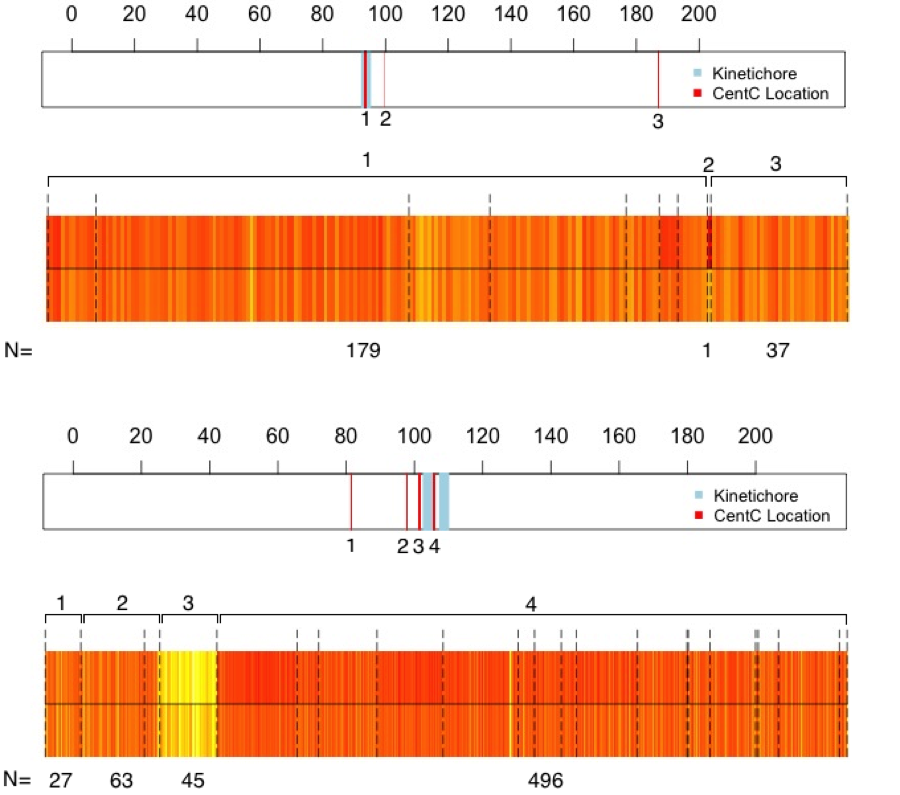
\includegraphics[width=1\textwidth]{heatmap.png}
\caption{CentC physical location and genetic relatedness for (a) chromosome 2 and (b) chromosome 5. \jri{need a and b labels } On the physical map, red lines show locations of numbered CentC clusters and blue blocks show the location of the active kinetichores.  Scale bar is in MB.  Below each physical map is shown a heatmap of genetic relatedness of each CentC to (top row) other copies within its island of tandem repeats delineated by dotted lines and (bottom row) all other copies on the chromosome.  Darker colors indicate higher relatedness.  The total number of CentC in each cluster is shown below the map.  
}
\label{heatmap}    
\end{figure}

The decreased genetic distance among CentCs in local clusters on chromosome 2 and 5 suggest that many of the genetic groupings discovered in our genome-wide analysis should correspond to local clusters of repeats. We see little evidence of this, however, as repeats within individual clusters are frequently found in different genetic groups as defined by principle component \jri{component or coordinate?} analysis (Figure \ref{pcoa}).  A comparison of all pairs of CentC sequences reveals a likely explanation: of the $\sim 74$ million possible pairs,  approximately 6 million share $\geq 2$ mutations different from the genome-wide consensus, likely grouping in genetic clusters despite their physical distance.  Looking at several triplets at random from our alignment confirms that two sequences in one PCoA assignment sometimes share greater pairwise identity than two sequences adjacent to one another in different PCoA groups.  A simple forward simulation (see Methods) suggests this pattern could be due entirely to homoplasy rather than long-distance movement of CentC repeats.  By stochastically applying mutations to an initially homogeneous group of repeat sequences, we find that plausible parameter values produce $\sim 10$ million pairs of repeats sharing $\geq 2$ mutations.      

\begin{figure}
% For two-column wide figures use
% Use the relevant command to insert your figure file.
\centering
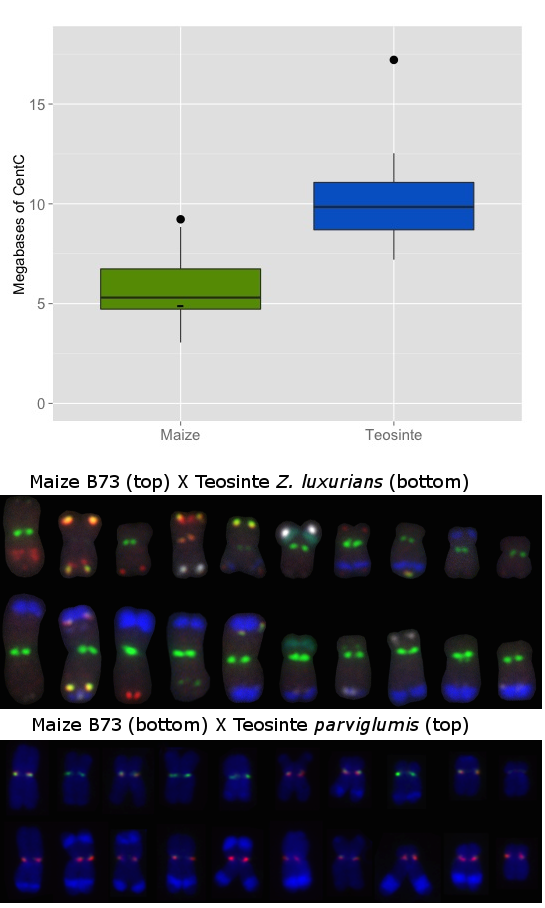
\includegraphics[width=1\textwidth]{Figure3_noedge}
\caption{(a) Mb of CentC in genomic libraries of maize and teosinte.  Box plots show data from \citet{Chia2012}.  Points show data for maize inbred B73 and the teosinte \emph{Z. luxurians} from \citet{Tenaillon2011}.  For comparison, the data point of maize inbred B73 in \citet{Chia2012} is shown with a tick mark on the box plot. (b) FISH images from an F1 hybrids between maize and the teosinte \emph{parviglumis}, and maize and the teosinte \emph{Z. luxurians}.  Upper row shows the karyotype for the teosinte and the lower row shows the maize karyotype.  Red=CentC, Green=CRM. 
}
\label{abundance}    
\end{figure}

\subsection*{Variation in CentC abundance in \emph{Zea}}

Shotgun sequence data from the maize HapMap v2 \citep{Chia2012}, reveals a significantly greater abundance of CentC in teosinte than in domesticated maize (p$<0.01$; Figure \ref{abundance}).   Further support for differences between maize and its wild relatives comes from shotgun sequence data from \emph{Z. luxurians} \citep{Tenaillon2011}.  Analysis of these data find nearly twice as much CentC in \emph{Z. luxurians} as the maize inbred B73.  To corroborate these results, we performed fluorescent in-situ hybridization of F1 crosses between inbred maize and teosinte to determine if cytological observations agreed with our sequencing findings.   FISH data supports our observation that the teosintes \emph{parviglumis} and \emph{Z. luxurians} have more CentC than inbred maize (Figure \ref{abundance}).  Using whole genome shotgun PacBio long reads, we further investigated the overall structure of repeats across the different \emph{Zea} species.  Percentages of the libraries showing tandem repeats did not differ greatly across the taxa (Supplementary Figure \ref{supp.pacbio}).

\section*{Discussion}
\label{discussion}

%% STUFF JEFF MAY ADD TO DISCUSSION
%Phylogenetic analysis of centromere repeats from a large number of eukaryotes found that repeat abundance evolves more rapidly than expected under a simple model of brownian motion \ref{Melters2012}. 

%While genome size (Poggio et al 1998), transposable elements (TEs) (Chia et al 2012), and heterochromatic knob content (Poggio et al 1998) are known to have changed greatly through domestication, little information exists as to how domestication has impacted centromeric repeats.  Previous cytogenetic work has identified considerable variation in centromere repeat content  between domesticated maize and its wild relatives Z. mays ssp. parviglumis,), Z. mays ssp. mexicana,, and Z. luxurians (hereafter parviglumis, mexicana, and luxurians) (Albert et al 2010). 

% It is likely that our empirical value is lower than our simulated value because we assume that all CentC copies have existed since the divergence event, while it is much more likely that age is high variable across copies.  Provided with such a large percentage of copies sharing mutations through homoplasy, we posit that it is possible for homoplasy, in the form of repeated mutations in different CentC copies, to drive our PCoA groupings.

Our study traces the changes in centromere repeat genetic relatedness across maize chromosomes to show how ancient tetraploidy and subsequent evolution has impacted centromeres.  Most interestingly, we show that most large arrays of CentC in the maize reference genome derive from maize1 subgenome, which is known to have lower gene loss and higher average expression than maize subgenome 2 \cite{Schnable2011}.  Regulatory microRNA’s are known to correspond to centromeric repeats \citep{ReinhartBartel2002}.  Therefore, it may be worthwhile to further investigate the potential correlation between centromere retention and gene expression as the phenomenon of higher expression of genes from one ancestor may be very common across plants (\emph{A. thaliana} \cite{Cheng2012} and \emph{Gossypium} Kapp and Wendel unpublished).  \pb{Two comments about this: first, its a terrible sentence so help make this better, because i think the point is really nice.  second, the best citations i found for cotton was an unpublished ref that is still not published from what i can gather.  advice? e.g. \url{http://www.plosone.org/article/info\%3Adoi\%2F10.1371\%2Fjournal.pone.0036442} also check out papers that cite Schabs: \url{http://scholar.google.com/scholar?cites=5313714612108479532&as_sdt=2005&sciodt=0,5&hl=en} } \jri{see journal policies, but citing unpublished usually kinda lame.} There are several possible explanations for the differential contribution of subgenome 1 to the diversity of CentC in the extant maize  genome. We put forth several hypotheses that may explain the strong bias for CentC to be located within a block from subgenome 1. Subgenome 2 may have had severely reduced quantities of CentC and therefore never contributed equally.  The CentC from subgenome 2 may have decayed rapidly and thus less of it remains.  Lastly, the CentC from subgenome 1 may have expanded in copy number since the allopolyploidy event.  Though we are unable to conclusively identify the reason, the lack of a large number of identical tandem duplicates  and lack of close proximity highest genetic relatedness pairs suggests that any large scale expansion of CentC has not been recent.  Also, CentC’s in subgenome 2 cluster do not appear to have accumulated excess mutation, suggesting that they are not decaying more rapidly than their subgenome 1 counterparts.  We therefore believe that it is most likely that the subgenomes had an unequal contribution of CentC at the formation of the allopolyploid, though more research about the ancient parents is required.  

We also explored how genetic relatedness between CentC’s correlated with location along the physical map.  According to our PCoA analyses, CentC copies across the genome do not form distinct genetic groups correlating with past origin (Figure \ref{pcoa}).  The lack of subgenome or chromosome grouping in modern CentC suggests a little differentiation between the repeats since the ancestral divergence.  Given the lack of a genome wide pattern, we also wanted to investigate genetic relatedness on individual chromosomes.  We hypothesized that most copies of CentC arose from local duplication rather than transposition, and therefore the genetic distance between CentC’s would be lowest across CentC’s within a large tandem array.  \pb{This part is ugly, and needs help} From the reference genome, we chose to investigate chromosomes 2 and 5, since they have been sequenced from end to end, allowing for inferences about the relationship between diversity and physical proximity \citep{Wolfgruber2009}.  Furthermore, the role of the repeat arrays on chromosomes 2 and 5 appear very different, as the largest array on chromosome 2 interacts with the kinetochore, while no array on chromosome 5 does \citep{Wolfgruber2009}.  We find that repeats on chromosomes 2 and 5 are most highly genetically related to neighboring copies (Figure \ref{heatmap}).  This relationship was recapitulated in analyses using SpaGeDi, where CentC’s within approximately 10-50KB of one another were more genetically similar (Supplemental Data \ref{Supp_SpagediChr02} and \ref{Supp_SpagediChr05}).  Though we did not investigate the relationship between CentC location and genetic similarity on the other chromosomes due to incomplete sequencing of centromeres, we observe that many CentC’s within an array fall into the same  significant grouping in our Tracy-Widom clustering analysis, suggesting that high local similarity of CentC’s is a genome-wide phenomenon.  This local relatedness suggests that most CentC is evolving through tandem duplication and not a long distance mechanism such as transposition that had been previously suggested \citep{Shi2010}.  Concerning chromosomes 2 and 5, the higher local relatedness of all CentC clusters regardless of presence within the kinetochore suggests that CentC interaction with kinetochore proteins does not have a detectable change on their rates of evolution.

When investigating why a pair of chromosomes on two different chromosomes are each other closest genetic relative, we revealed that homoplasy in mutations is common across CentC variants.  We suggest that copies of CentC are sufficiently old within the genome that homoplasious mutations cause physically distant CentC’s to be highly genetically related.  Importantly, we also do not see PCoA group capturing full clusters across chromosomes in a way that would be consistent with retrotransposition. We speculate that a vast majority of the CentC’s exist as a result of very old duplications meaning that mutations have had a long time to accumulate. Roughly 80\% of the CentC repeats have their closest genetic relative on the same chromosome, an observation we would expect if CentC’s on a chromosome share ancestry.  However, only 14\% of closest genetic pairs are found within 10KB of each other, suggesting that their tandem duplication is old and that most CentC’s have persisted within the genome for a long time. \pb{This is an important sentence, and I can’t seem to get it to communicate my point properly.  perhaps because im making too many points}

When studying CentC changes through domestication, our findings show that the repeat has experienced a decrease in copy number over time without a noticeable change in the structure of the repeat arrays. Using PacBio long read sequencing, we confirm genome-wide the observation we see on chromosomes 2 and 5, that most copies of CentC exist in large tandem arrays in all \emph{Zea} taxa.  From short read sequencing data, we show that modern maize has reduced genomic abundance of CentC when compared to the teosintes, a finding confirmed through FISH (Figure \ref{abundance}).  Both teosintes within the species \emph{mays} and its sister species \emph{luxurians} have elevated levels of CentC.  Lower levels of centromere repeats in inbred maize contrasts previous studies that characterized the changing abundance of other common repeats.  For example, the abundance of most transposable element families increased after domestication \citep{Chia2012}.  Knowing that TE abundance increases in domesticated maize, we might have expected CentC content to increase as well if centromere size had to expand alongside most other repetitive content.  Alternatively, due to their structural role in kinetichore formation, we might have also expected centromere repeats to be largely excluded from the genome wide fluctuations in repetitive content assuming that selection exists to maintain centromere size.  Instead, the decrease in CentC content may indicate an active process of removing CentC.  We hypothesize that the removal of CentC content may correlate with genome size, as the sharp decrease in knob content through domestication actually led to an overall smaller genome size in inbred maize. The correlation between  functional  centromere size and genome size has been observed in grass species \citep{Zhang2012}.  Further investigation would be required to discover whether only those copies of CentC outside of the active kinetochore are being deleted.

We also sought to further characterize the chromosome specific repeat cent4 \citep{Page2001}.  Previous work showed that Cent4 probes lagged behind CentC probes in cell division \citep{Jiang2002}, suggesting that the repeat is not involved in the active kinetochore and rather located in the pericentromere.  A lack of enrichment of cent4 in ChIP data agrees with a pericentromeric location.  Using the published cent4 sequences, we identify the cent4 repeat as the LTR retrotransposon RLX\_sela in the transposable element database \citep{Baucom2009}.  Characterization of the TE consensus sequence shows that it contains repetitive motifs with homology to both knob and telomere repeats.  It lacks any of the protein sequences necessary for autonomous transposition, such as GAG and POL complexes.  Previous work in rice has documented the presence of nonautonomous LTR retrotransposons  in or near the centromere \citep{Jiang2002}.  However, the RLX\_sela sequence also appears to be missing some of the necessary primer binding sites that would distinguish it as a nonautonomous TE, suggesting that it may be a tandem repeat, and further sequencing of the region will be required to uncover the role of cent4.   Given that the centromere and pericentromere on chromosome 4 show signs of strong selection during domestication \citep{Hufford2012}, it is plausible that the increase in abundance of Cent4 seen in domesticated maize is due to the effects of linked selection on a locus important for domestication rather than novel insertions or duplications. 

In conclusion, our study pairs bioinformatics and cytology to validate observations of decreasing centromere repeat content through maize domestication.  We show that patterns of CentC similarity are consistent with tandem duplications and maize’s allopolyploid history has left no significant differentiation between CentC’s from the different maize subgenomes. We also identify the chromosome 4 specific repeat, cent4, as the TE RLX\_sela and show that it has increased through domestication, unlike a majority of the other TEs \citep{Chia2012}.    

\jri{quick scan of the references looks OK, but do double check format etc.}

\begin{acknowledgements}
We wish to thank Pacific Biosciences for sequencing resources.  We thank Siddharth Bhadra-Lobo, Vince Buffalo, Anne Lorant, Gernot Presting, Lauren Sagara, Michelle Stitzer, and NSF summer exchange program interns Cesar Alvarez Mejia, Aurelio Hernandez Bautista for advice and helpful discussion. This project was funded by NSF grant IOS-0922703.
\end{acknowledgements}

% BibTeX users please use one of
\bibliographystyle{spbasic}      % basic style, author-year citations
%\bibliographystyle{spmpsci}      % mathematics and physical sciences
%\bibliographystyle{spphys}       % APS-like style for physics
\bibliography{refcentc}   % name your BibTeX data base

\newpage

\section*{Supplemental Material}

\begin{figure}[h!]
% For two-column wide figures use
% Use the relevant command to insert your figure file.
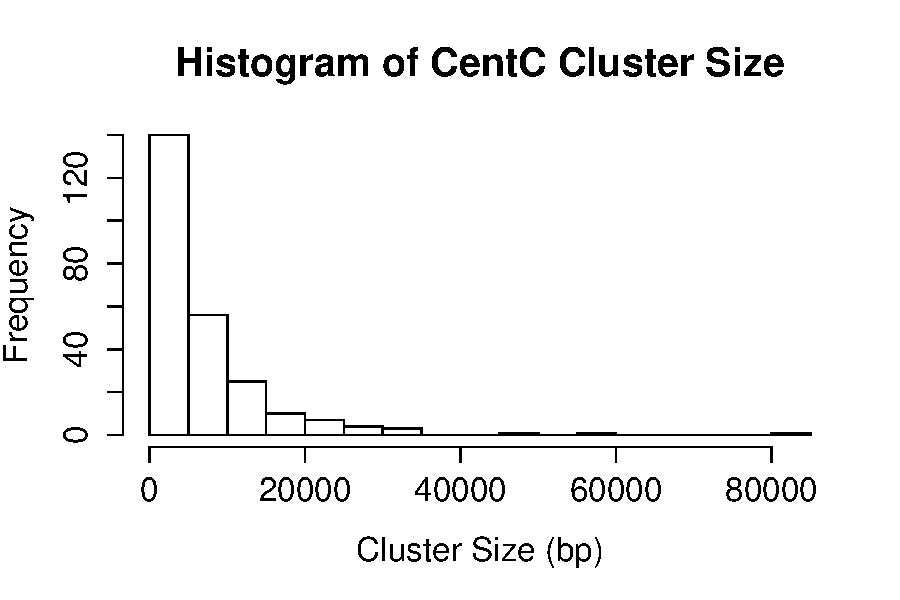
\includegraphics[width=1\textwidth]{Supp_clusterhist}
\setcounter{figure}{0}
\caption{CentC cluster size across all chromosomes.}
\label{Supp_clusterhist}    
\end{figure}

\begin{figure}[h!]
% For two-column wide figures use
% Use the relevant command to insert your figure file.
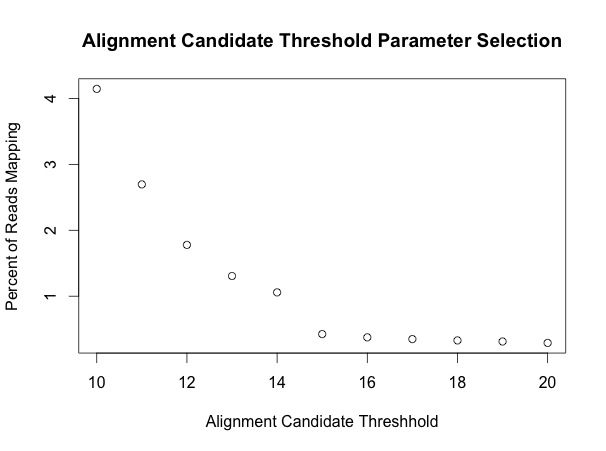
\includegraphics[width=1\textwidth]{Suppl_ACT_Seln.jpeg}
\setcounter{figure}{0}
\caption{Parameter selection for Alignment Candidate Threshold (ACT) for Mosaik.  All other parameters were kept constant while ACT was changed.  ACT was the parameter for which a non-linear pattern was observed.  We selected to use an ACT of 15, the value for which we observed the greatest relative decrease between total percent mapping values.  The sharp change suggests that, at a lower ACT, we may be mapping a non-CentC element to our reference.}
\label{Supp_MPS}    
\end{figure}

\begin{figure}[h!]
% For two-column wide figures use
% Use the relevant command to insert your figure file.
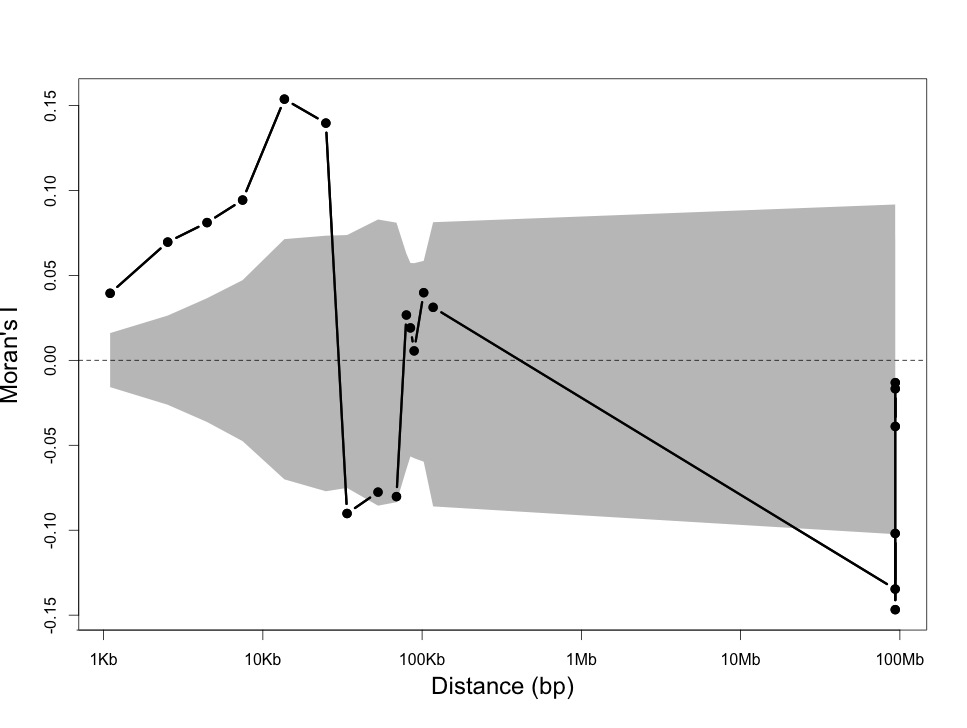
\includegraphics[width=1\textwidth]{Suppl_Chr02_Rspagedi.jpeg}
\caption{Measure of Moran's I for Chromosome 2.  Gray areas show the confidence interval, calculated using permutations of genetic distance.}
\label{Supp_SpagediChr02}    
\end{figure}

\begin{figure}[h!]
% For two-column wide figures use
% Use the relevant command to insert your figure file.
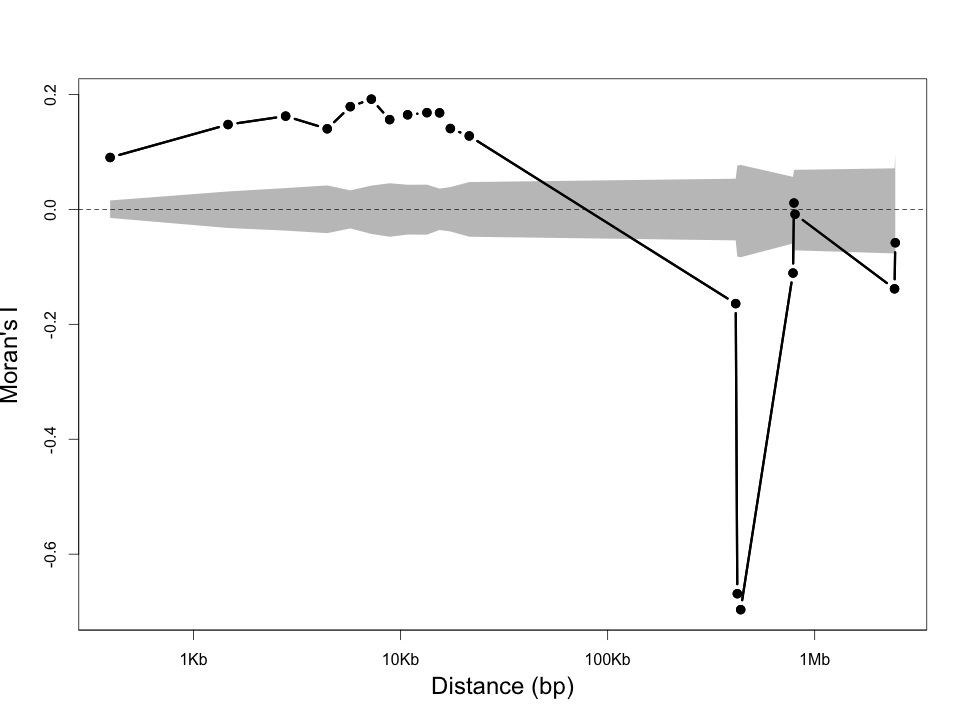
\includegraphics[width=1\textwidth]{Suppl_Chr05_Rspagedi.jpeg}
\caption{Measure of Moran's I for Chromosome 5.  Gray areas show the confidence interval, calculated using permutations of genetic distance.}
\label{Supp_SpagediChr05}    
\end{figure}

\begin{figure}[h!]
% For two-column wide figures use
% Use the relevant command to insert your figure file.
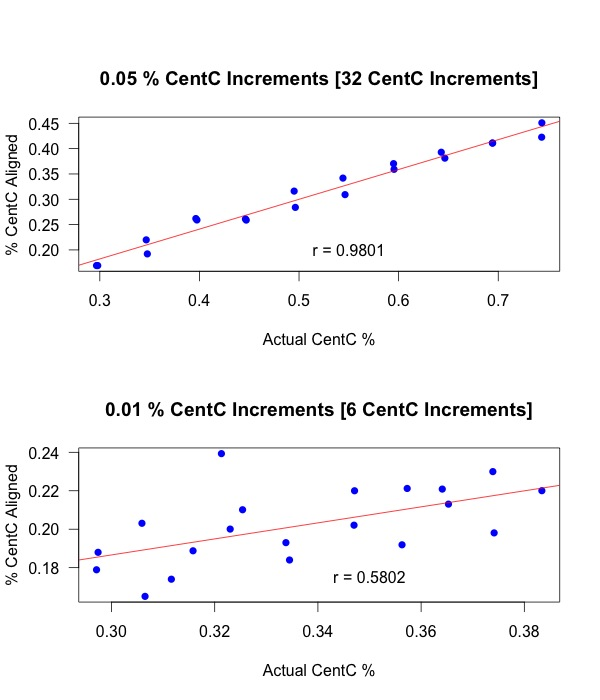
\includegraphics[width=1\textwidth]{AccuracyTest_2graphs.jpeg}
\caption{Graphs showing our ability to capture changes in CentC repeat abundance under constant genome size.  We simulated 10MB of DNA with varying CentC content and  simulated Illumina reads from the DNA.  Reads were mapped with our Mosaik pipeiline, and several simulations at each percentage of genomic content were performed.}
\label{Supp_Accuracy}    
\end{figure}

\begin{table}[h!]
\caption{CentC Occurence Count In Maize RefGenv2}
\label{supp.occurence}       % Give a unique label
% For LaTeX tables use
\begin{tabular}{ll}
\hline\noalign{\smallskip}
Occurrences &  Number of CentC's\\
\noalign{\smallskip}\hline\noalign{\smallskip}				
1	&8259\\
2	&1233\\
3	&263\\
4	&89\\
5	&31\\
6	&13\\
7	&7\\
8	&0\\
9	&0\\
10	&1\\
\noalign{\smallskip}\hline
\end{tabular}
\end{table}


% For tables use
\begin{table}[h!]
\caption{PacBio Read Counts and Tandem CentC}
\label{supp.pacbio}       % Give a unique label
% For LaTeX tables use
\begin{tabular}{llll}
\hline\noalign{\smallskip}
Maize Line & Reads over 600bp & Reads with $\geq 4$ CentC & \% Reads Showing Tandem CentC \\
\noalign{\smallskip}\hline\noalign{\smallskip}				
B73	& 237995	& 30	& 0.030252736	\\
\emph{luxurians}		&156964	&	79	&	0.050330012	\\
\emph{mexicana}	 	&141939 	&	150	&	0.1056792	\\
\emph{parviglumis}	&227050	& 89		&	0.039198414	\\
\noalign{\smallskip}\hline
\end{tabular}
\end{table}

% For tables use
\begin{table}[h!]
\caption{ChIP Reads mapping to Unassembled from different Oat-Maize Addition (OMA) Lines}
\label{supp.gaby}       % Give a unique label
% For LaTeX tables use
\begin{tabular}{llll}
\hline\noalign{\smallskip}
File Key & Maize Chr & Percent Reads Aligning to Unassembled BACs\\
\noalign{\smallskip}\hline\noalign{\smallskip}				
JJ1BU (OMA 6.34) & 6 & 21.35\\
JJ1BR (OMA 1.36) & 1 & 15.56\\
JJ1CF (OMA 9.41) & 9 & 6.16\\
JJ1CH (OMA 8.05) & 8 & 6.69\\
JJ1CG (OMA 10.26) & 10 & 9.21\\
JJ1CI (OMA 8.05) & 8 & 8.5\\
\noalign{\smallskip}\hline
\end{tabular}
\end{table}


\pagebreak
 \begin{longtable}[c]{|c|c|c|c|c|c|c|c|c|c|c|}
 \caption{Heirarchical clustering group assignment for copies of CentC, sorted by chromosome.  The number of CentC's from each chromosome is represented in the table.\label{long}}\\ 
\hline

\hline
Group & Chr01 & Chr02 & Chr03 & Chr04 & Chr05 & Chr06 & Chr07 & Chr08 & Chr09 & Chr10\\
 \hline
 \endfirsthead

\hline
\multicolumn{1}{|c|}{Table \ref{long} Continued}\\
\hline
Group & Chr01 & Chr02 & Chr03 & Chr04 & Chr05 & Chr06 & Chr07 & Chr08 & Chr09 & Chr10\\ 
\hline
 \endhead %Jeff, I absolutely cannot get this stupid repeated header thing to work.  Any guesses as to why its not?  

 \hline
 \endhead
 
 \hline
 \endfoot
 
 \hline
 \endlastfoot
 
1 & 59 & 10 & 19 & 15 & 28 & 0 & 101 & 31 & 23 & 51\\
2 & 98 & 0 & 0 & 0 & 1 & 0 & 1 & 0 & 1 & 0\\
3 & 149 & 0 & 0 & 0 & 0 & 0 & 1 & 0 & 1 & 1\\
4 & 125 & 45 & 105 & 64 & 72 & 4 & 494 & 117 & 155 & 303\\
5 & 6 & 0 & 0 & 0 & 0 & 0 & 0 & 0 & 0 & 0\\
6 & 1 & 0 & 1 & 0 & 0 & 0 & 0 & 0 & 0 & 0\\
7 & 234 & 0 & 0 & 0 & 0 & 0 & 0 & 0 & 0 & 0\\
8 & 0 & 0 & 0 & 1 & 0 & 0 & 427 & 0 & 0 & 4\\
9 & 0 & 0 & 0 & 0 & 0 & 0 & 0 & 1 & 28 & 81\\
10 & 0 & 0 & 0 & 0 & 0 & 0 & 0 & 0 & 152 & 38\\
11 & 0 & 0 & 0 & 0 & 0 & 0 & 91 & 0 & 0 & 0\\
12 & 242 & 33 & 115 & 0 & 0 & 0 & 8 & 2 & 0 & 1\\
13 & 0 & 0 & 0 & 0 & 0 & 0 & 0 & 0 & 0 & 0\\
14 & 20 & 2 & 17 & 0 & 7 & 0 & 340 & 2 & 3 & 0\\
15 & 28 & 0 & 0 & 0 & 0 & 0 & 0 & 0 & 0 & 0\\
16 & 65 & 0 & 0 & 0 & 0 & 0 & 0 & 0 & 0 & 0\\
17 & 2 & 0 & 0 & 0 & 0 & 0 & 0 & 0 & 0 & 0\\
18 & 113 & 0 & 0 & 0 & 0 & 0 & 0 & 0 & 0 & 0\\
19 & 225 & 0 & 0 & 0 & 0 & 0 & 0 & 0 & 0 & 0\\
20 & 135 & 0 & 0 & 0 & 0 & 0 & 0 & 0 & 0 & 0\\
21 & 200 & 62 & 104 & 0 & 0 & 0 & 1 & 0 & 1 & 0\\
22 & 0 & 0 & 0 & 0 & 8 & 0 & 122 & 0 & 0 & 0\\
23 & 7 & 0 & 0 & 3 & 0 & 0 & 98 & 205 & 123 & 3\\
24 & 17 & 0 & 89 & 0 & 0 & 0 & 0 & 0 & 0 & 0\\
25 & 0 & 1 & 0 & 0 & 0 & 0 & 198 & 0 & 0 & 0\\
26 & 11 & 64 & 22 & 0 & 0 & 0 & 0 & 0 & 0 & 0\\
27 & 6 & 0 & 140 & 47 & 0 & 0 & 0 & 0 & 0 & 0\\
28 & 0 & 0 & 169 & 47 & 0 & 0 & 0 & 0 & 0 & 0\\
29 & 0 & 0 & 0 & 0 & 0 & 0 & 0 & 0 & 0 & 151\\
30 & 0 & 0 & 0 & 66 & 283 & 0 & 1 & 0 & 0 & 0\\
31 & 0 & 0 & 0 & 87 & 202 & 0 & 0 & 0 & 0 & 0\\
32 & 0 & 0 & 0 & 0 & 25 & 0 & 0 & 0 & 0 & 0\\
33 & 0 & 0 & 0 & 0 & 0 & 12 & 55 & 0 & 0 & 0\\
34 & 0 & 0 & 0 & 0 & 2 & 16 & 213 & 0 & 0 & 0\\
35 & 0 & 0 & 0 & 0 & 0 & 0 & 56 & 0 & 0 & 0\\
36 & 0 & 0 & 0 & 0 & 0 & 0 & 217 & 0 & 0 & 0\\
37 & 0 & 0 & 0 & 0 & 0 & 0 & 25 & 0 & 0 & 0\\
38 & 0 & 0 & 0 & 0 & 3 & 0 & 248 & 1 & 19 & 1\\
39 & 0 & 0 & 0 & 0 & 0 & 0 & 60 & 80 & 0 & 0\\
40 & 0 & 0 & 0 & 0 & 0 & 0 & 182 & 0 & 0 & 0\\
41 & 0 & 0 & 0 & 0 & 0 & 0 & 90 & 0 & 0 & 0\\
42 & 0 & 0 & 0 & 0 & 0 & 0 & 58 & 0 & 0 & 0\\
43 & 0 & 0 & 0 & 0 & 0 & 0 & 87 & 0 & 0 & 0\\
44 & 0 & 0 & 0 & 0 & 0 & 0 & 22 & 135 & 1 & 0\\
45 & 0 & 0 & 0 & 0 & 0 & 0 & 0 & 85 & 98 & 0\\
46 & 0 & 0 & 0 & 0 & 0 & 0 & 0 & 0 & 150 & 1\\
47 & 0 & 0 & 0 & 0 & 0 & 0 & 0 & 0 & 0 & 254\\
48 & 0 & 0 & 0 & 0 & 0 & 0 & 0 & 0 & 70 & 0\\
49 & 0 & 0 & 0 & 0 & 0 & 0 & 0 & 0 & 193 & 1\\
50 & 0 & 0 & 0 & 0 & 0 & 0 & 0 & 0 & 93 & 0\\
51 & 0 & 0 & 0 & 0 & 0 & 0 & 0 & 0 & 2 & 62\\
52 & 0 & 0 & 0 & 0 & 0 & 0 & 2 & 0 & 0 & 311\\
53 & 0 & 0 & 0 & 0 & 0 & 0 & 0 & 0 & 0 & 168\\
54 & 0 & 0 & 0 & 0 & 0 & 0 & 0 & 0 & 0 & 112\\
55 & 0 & 0 & 0 & 0 & 0 & 0 & 0 & 0 & 0 & 42\\
56 & 0 & 0 & 0 & 0 & 0 & 0 & 2 & 0 & 0 & 226\\
57 & 0 & 0 & 0 & 0 & 0 & 0 & 0 & 0 & 0 & 66\\
58 & 0 & 0 & 0 & 0 & 0 & 0 & 0 & 0 & 0 & 56\\

 \end{longtable}



\end{document}
% end of file template.tex

